\section{\pepit}
PEPIT est né le 15 mai 2004 à Mouscron en Belgique. Il s'agissait, à l'époque, de créer une plateforme numérique d'échange d'exercices entre 5 écoles primaires et le premier degré d'une école secondaire.


Le projet a connu différentes évolutions au fil du temps, la troisième version du site est actuellement en ligne. Cette dernière version contient plus de 1250 exercices en ligne, la variété et la qualité de nos exercices sont appréciées les mois "scolaires" par plus de 200.000 "visiteurs uniques".
%% ************************************************** %
\section{Et nous, que vient-on faire là dedans ?}
Actuellement, le pepit.be est un portail d'accès à des applications Flash, où il est possible de jouer directement sur le site ou de télécharger le jeu sur l'ordinateur (PC ou MAC).


Notre objectif est de réaliser une application Android, destinée principalement aux tablettes. Cette application regroupera les jeux, mais ils ne redirigeront pas vers une application en Flash mais vers une version Android, les jeux devront être redéveloppés. Celle-ci sera utilisée pour l'apprentissage des enfants, il faut donc faire attention à l'ergonomie de l'application.


Nous avons la charge de d'étudier l'actuel portails, concevoir, développer l'application Android. Et comme challenge supplémentaire, une API qui permettrait de construire des jeux sans passer par \java{}.

%% ************************************************** %
%% Présentation de l'existant

\section{L'existant}
Actuellement un site internet est en place, c'est un portail de jeux au format flash. Chaque jeu est créé à la main de façon artisanal.

\begin{figure}[H]
\begin{center}
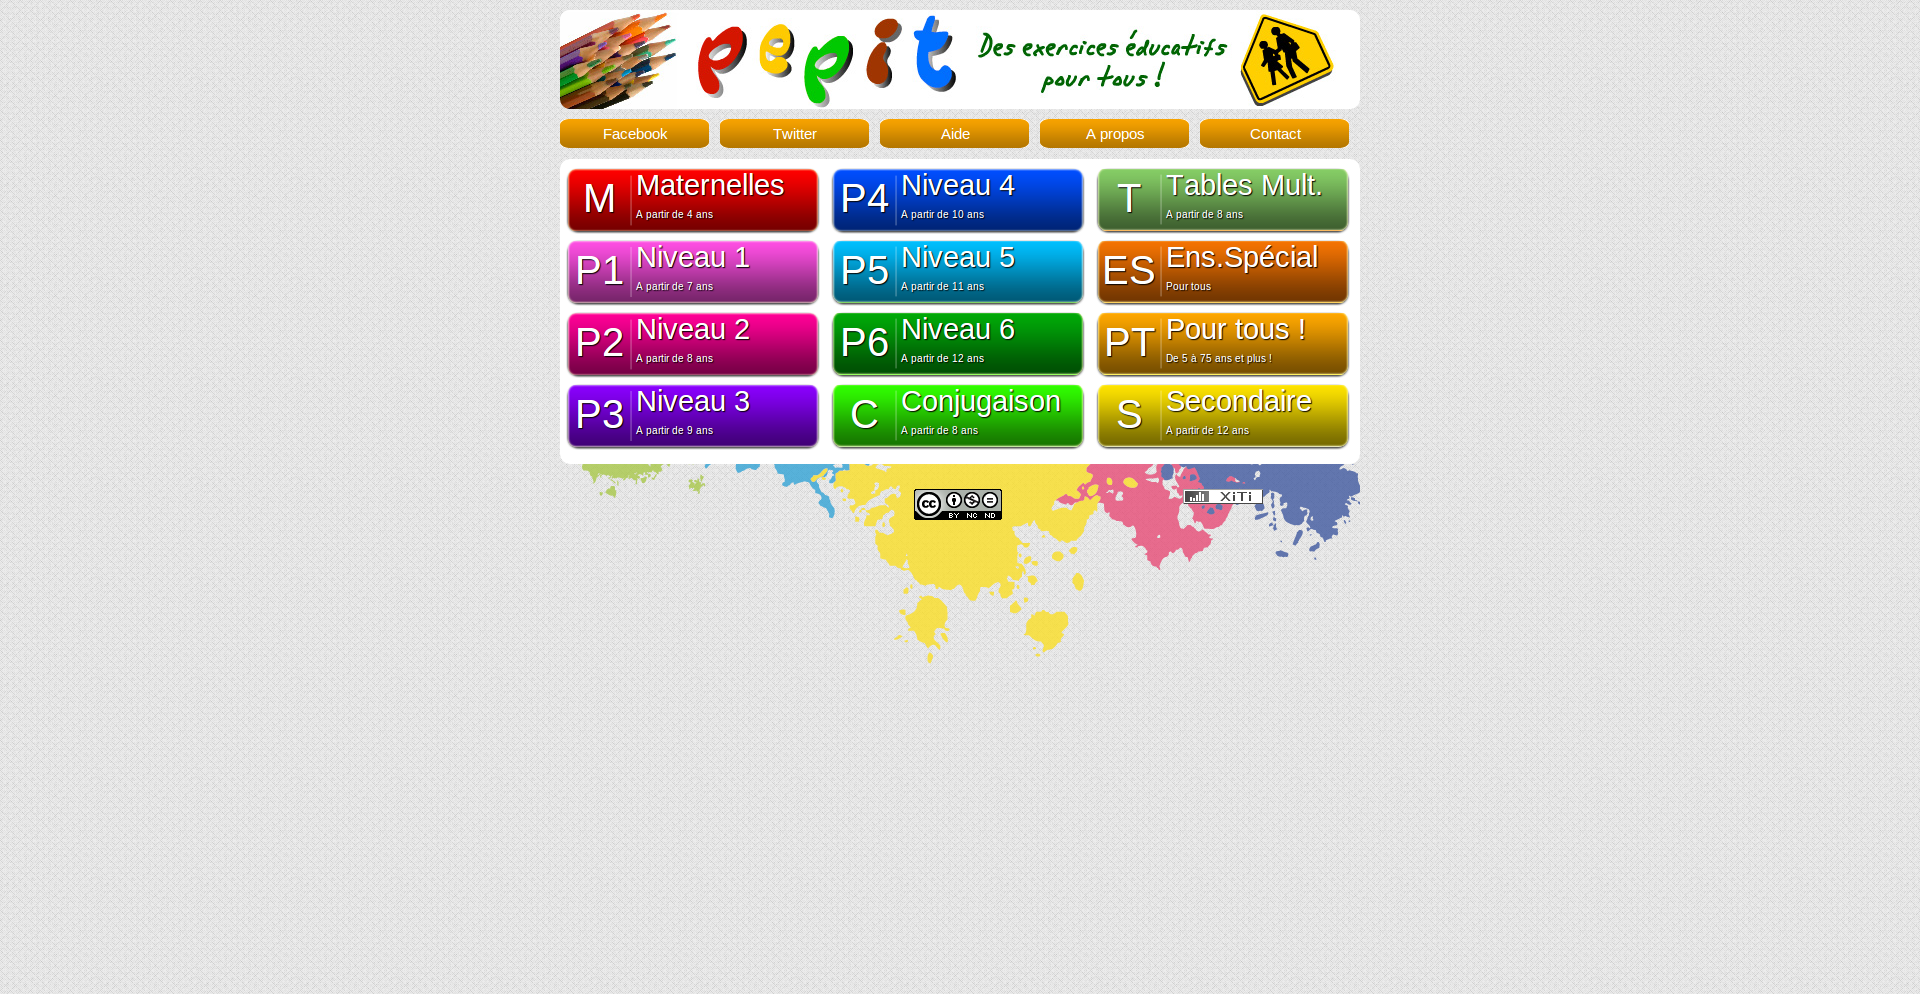
\includegraphics[width=15cm]{images/pepit_be_homepage}
\end{center}
\caption{Pepit Mobil - Page d'accueil}
\label{Pepit Mobil - Page d'accueil}
\end{figure}

\begin{figure}[H]
\begin{center}
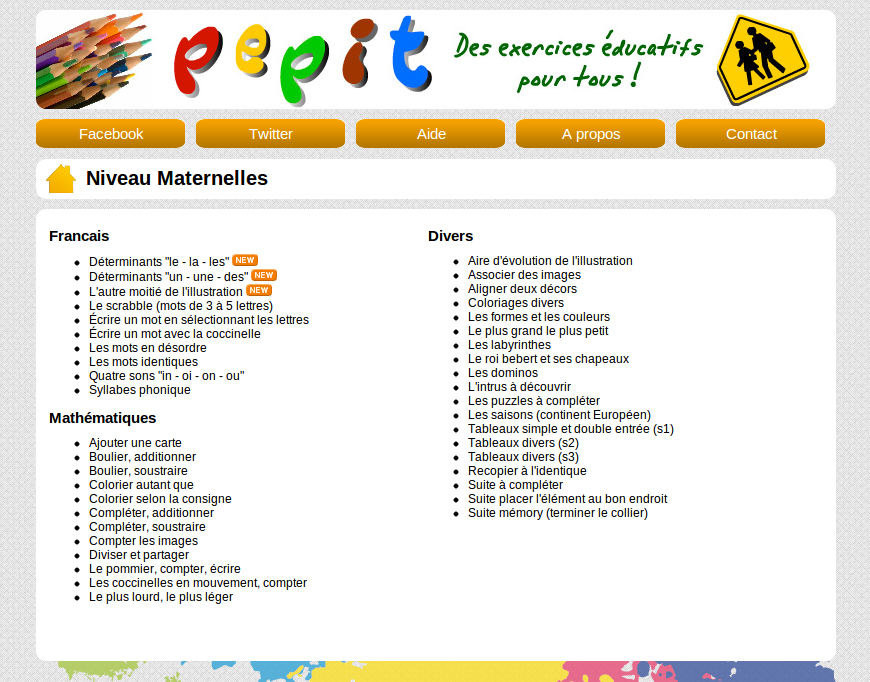
\includegraphics[width=15cm]{images/pepit_be_list}
\end{center}
\caption{Pepit Mobil - Liste des thèmes}
\label{Pepit Mobil - Liste des thèmes}
\end{figure}

\begin{figure}[H]
\begin{center}
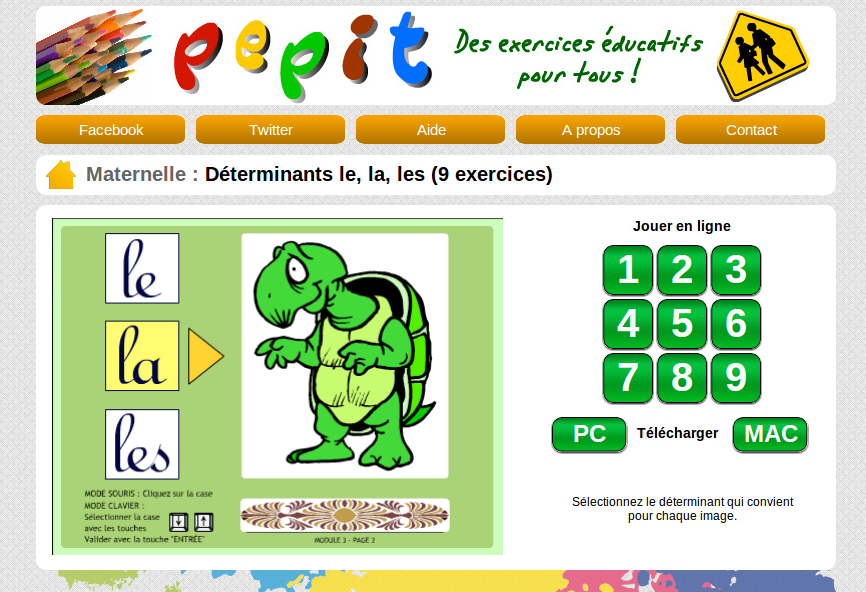
\includegraphics[width=15cm]{images/pepit_be_modules}
\end{center}
\caption{Pepit Mobil - Sélection d'un module}
\label{Pepit Mobil - Sélection d'un module}
\end{figure}

\begin{figure}[H]
\begin{center}
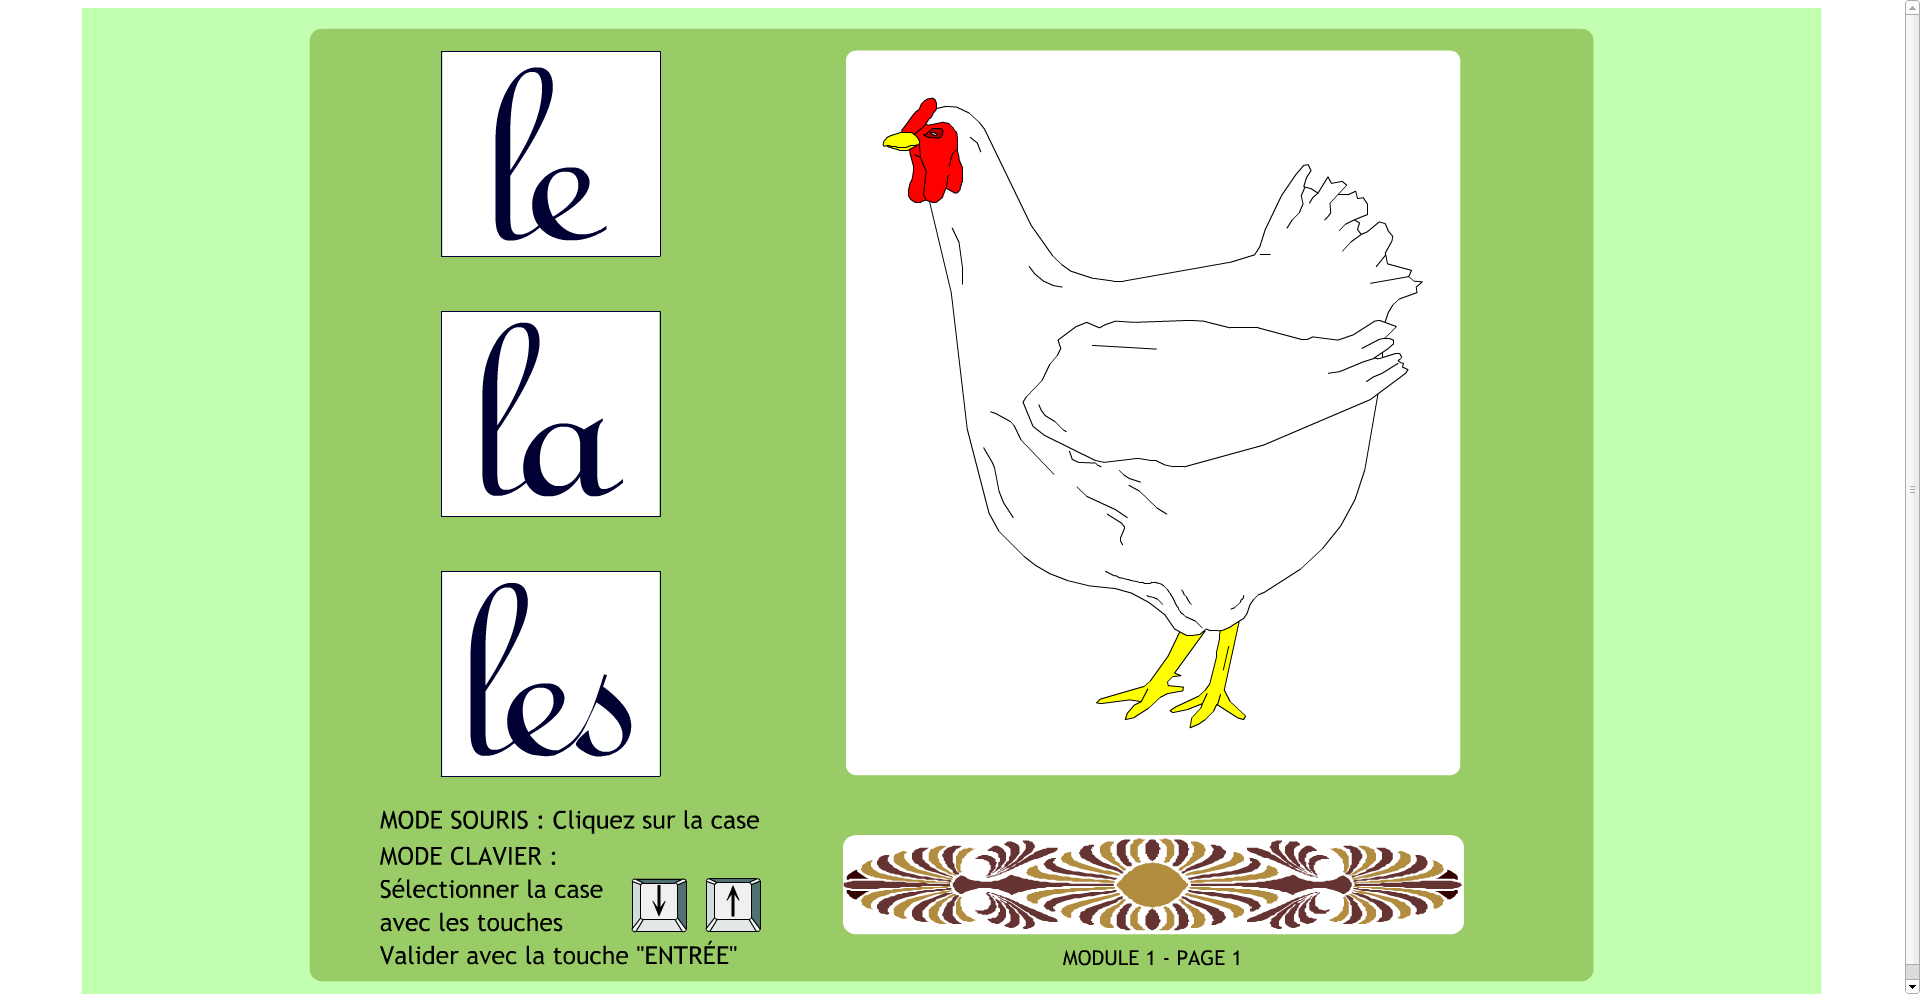
\includegraphics[width=15cm]{images/pepit_be_practice}
\end{center}
\caption{Pepit Mobil - Un exercice}
\label{Pepit Mobil - Un exercice}
\end{figure}